\section{Introduction}
\label{sec:introduction}

% state the learning objective 
The objective of this laboratory assignment is to convert an alternated current signal with 230V, 50Hz, to a 12V direct current source, using an envelope detector and a voltage regulator.\par
The circuit was simulated in NGSpice, with a theoretical prediction in Octave. The merit of this work is related to the ripple and cost of the components: the less ripple and the lower the cost, the higher the merit. In this assignment, the merit obtained was aproximately 0,26. 

The merit is calculated using the following expression:\par
\begin{equation}
    M = \frac{1}{Cost(ripple(v_0)+average(v_0-12)+10^{-6})}
\end{equation}\par
Where: \par
Cost = cost of resistors + cost of capacitors + cost of diodes \par
Cost of Resistors = 1 monetary unit per kOhm \par
Cost of capacitor = 1 monetary unit per $\mu$ F \par
Cost of diodes = 0.1Monetary units per diode \par
The circuit is shown below in figure (Fig.\ref{fig:circuito}): \par

\begin{figure}[H]
\centering
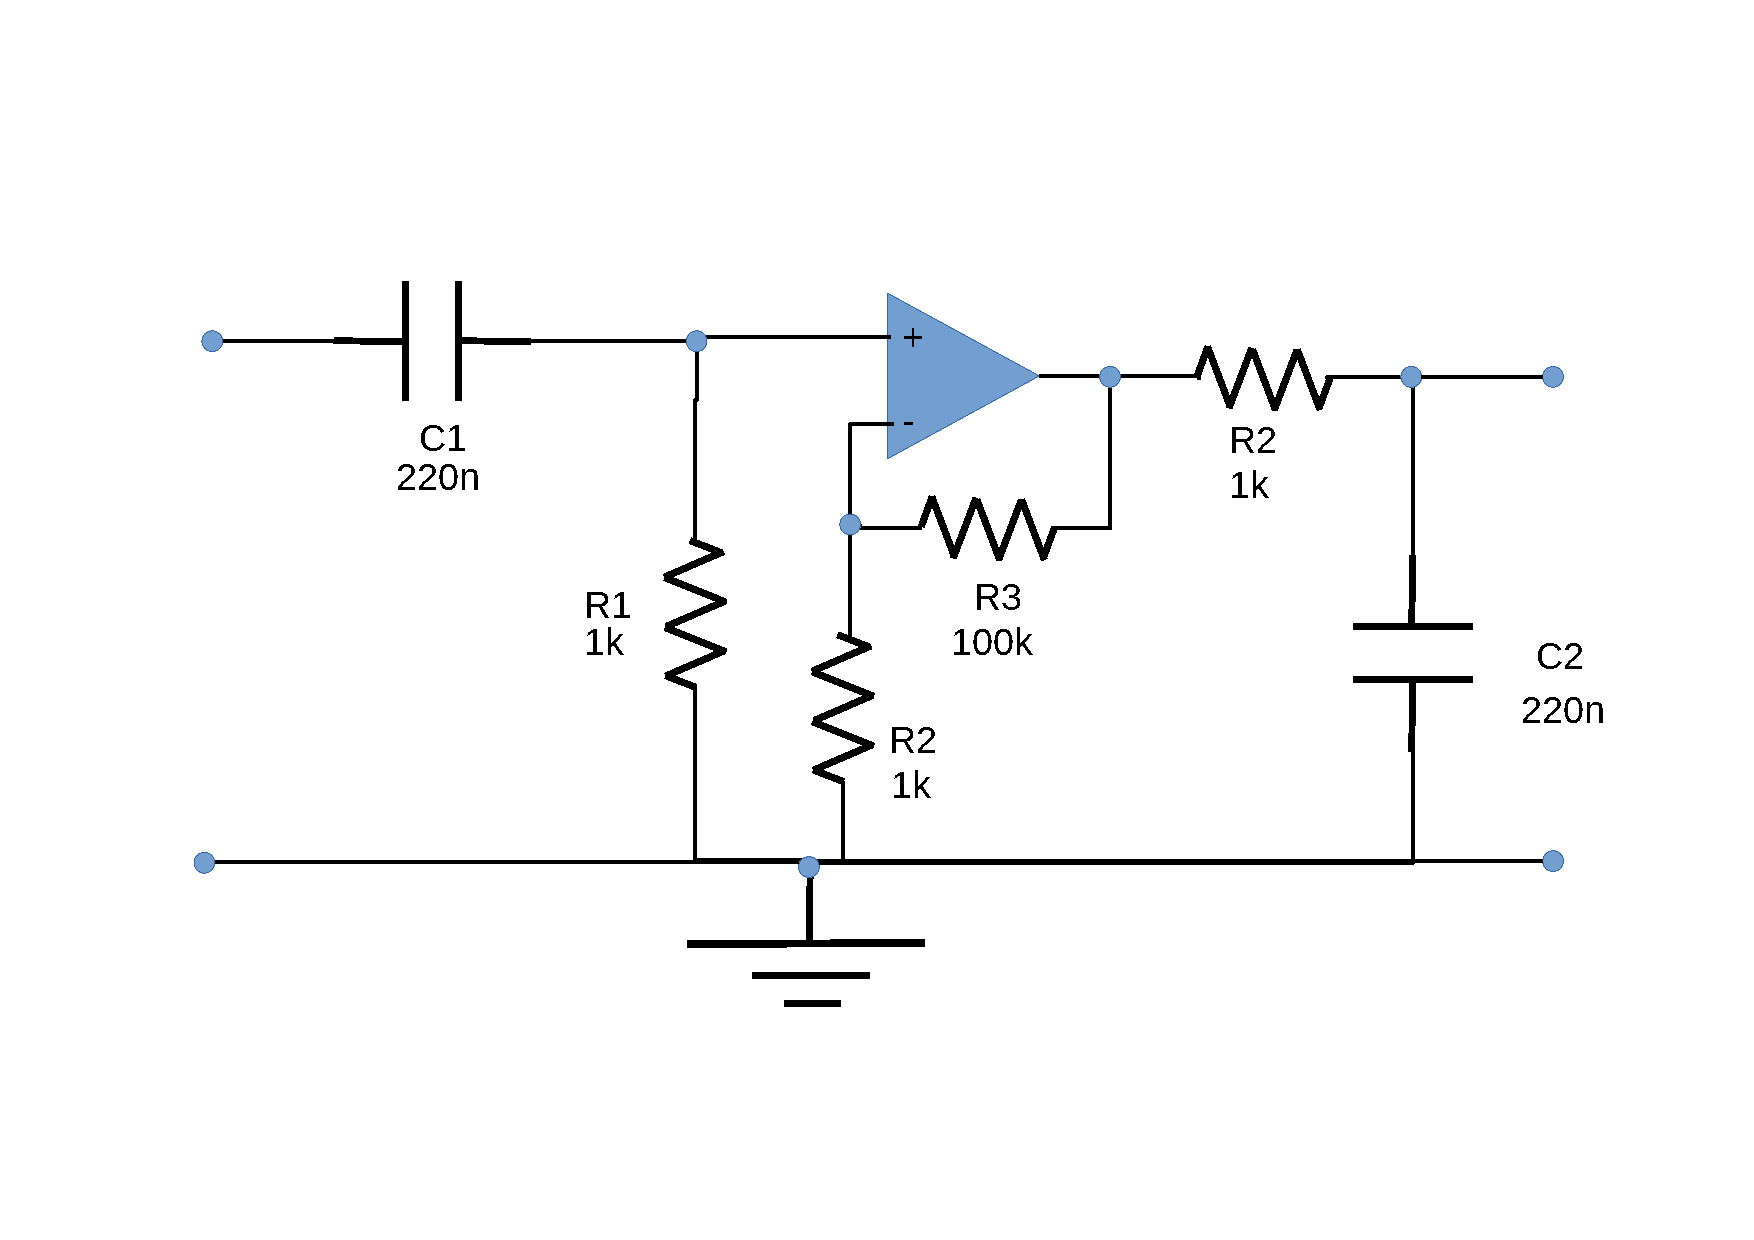
\includegraphics[scale=0.6]{circuito}
\caption{Final circuit}
\label{fig:circuito}
\end{figure}

The individual costs of the components used: \par
- Diodes - cost: 2.3MU; \par
- Capacitor - 26MU; \par
- Resistances - 33.15MU. \par

The data used was the following:

\begin{center}
  \begin{tabular}{ | c | c | }
    \hline    
    {\bf Name} & {\bf Value} \\ \hline
    $R_1$ & 26 k$\Omega$ \\ \hline 
    $R_2$ & 7.15 k$\Omega$ \\ \hline 
    $C$ & 26 $\mu$S \\ \hline
    Diodes & 23 Units \\ 
    \hline
  \end{tabular}
\end{center}